\begin{minipage}{0.35\textwidth}
    \begin{figure}[h]
    \centering
    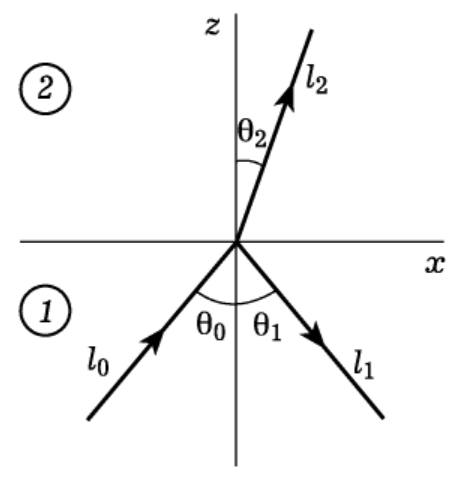
\includegraphics[width=1\textwidth]{images/brust.png}
    \caption{0 stands for a in-going wave, 1 stands for a transmitted wave, 2 stand for a reflected wave.}
    %\label{fig:}
\end{figure}
\end{minipage}
\hfill
\begin{minipage}{0.55\textwidth}
	The angular encounter of the light with a plane is described as
	\begin{equation}
		\begin{aligned}
			&R_\perp = \frac{sin^2(\theta_2 - \theta_0)}{\sin^2(\theta_2 + \theta_0)},\\
			\hspace{1 cm}
			&R_\parallel = \frac{\tg^2(\theta_2 - \theta_0)}{\tg^2(\theta_2 + \theta_0)}.	
		\end{aligned}
	\end{equation}    
\end{minipage}

